%# -*- coding: utf-8-unix -*-
%%==================================================
%% chapter01.tex for SJTU Master Thesis
%%==================================================

%\bibliographystyle{sjtu2}%[此处用于每章都生产参考文献]
\chapter{AKI算法}
\label{chap:Alg}

为了确定一个子密钥集合$K$的实际密钥信息,我们需要一个算法来计算AKI的值并得到一些可能的实际密钥信息集合。
黄佳琳博士在\citen{Huang_2014}中提出了一个自动化搜索密钥信息泄露的工具,但该工具设计的算法是一个贪心算法,只能计算出AKI的一个合理上界,无法得到真实的AKI值。
一个AKI的合理上界可以用来进行攻击可能性的分析,但无法用来实际分析一个密钥编排方案的强弱。
Lin等人在\citen{lin2016automatic}中提出了一种对密钥桥技术(Key-Bridging Technique\citen{dunkelman2010improved})的自动化搜索算法,但时间复杂度极高,无法进行大量不同$K$的计算,并且也存在一些反例无法计算(后文中将会提到一个反例)。
因此,现有的AKI算法由于只能给出AKI的一个合理上界,只能用于攻击分析,无法用来分析密钥编排方案的强弱好坏,也不能用来改进密钥编排方案的设计。
本章将会介绍一种全新的基于图论的AKI算法,将会在多项式时间复杂度内计算出真实的AKI值。

\section{单轮加密的AKI}
\label{Bigraph}
在介绍完整的AKI算法之前,我们首先从简化版的问题开始考虑——仅有一轮加密时的AKI计算。
我们假设子密钥集合$K$全部集中在第$r$轮上,然后只考虑$r$轮和$r-1$轮两轮之间的依赖关系。
为了解决这个问题,我们将使用图论中二分图的思想来将编排方案、密钥比特、依赖关系等参数量化成图,进而将AKI的计算转化为一个图论的问题。
\begin{defn}[二分图]
    设$G(V,E)$是一个无向图,如果顶点集合$V$可以分割为两个互不相交的子集$A,B$且图中每条边的两个顶点分别属于不同的子集,则称$G$为一个二分图,可记为$G(A,B,E)$。
\end{defn}
\begin{figure}
    \centering
    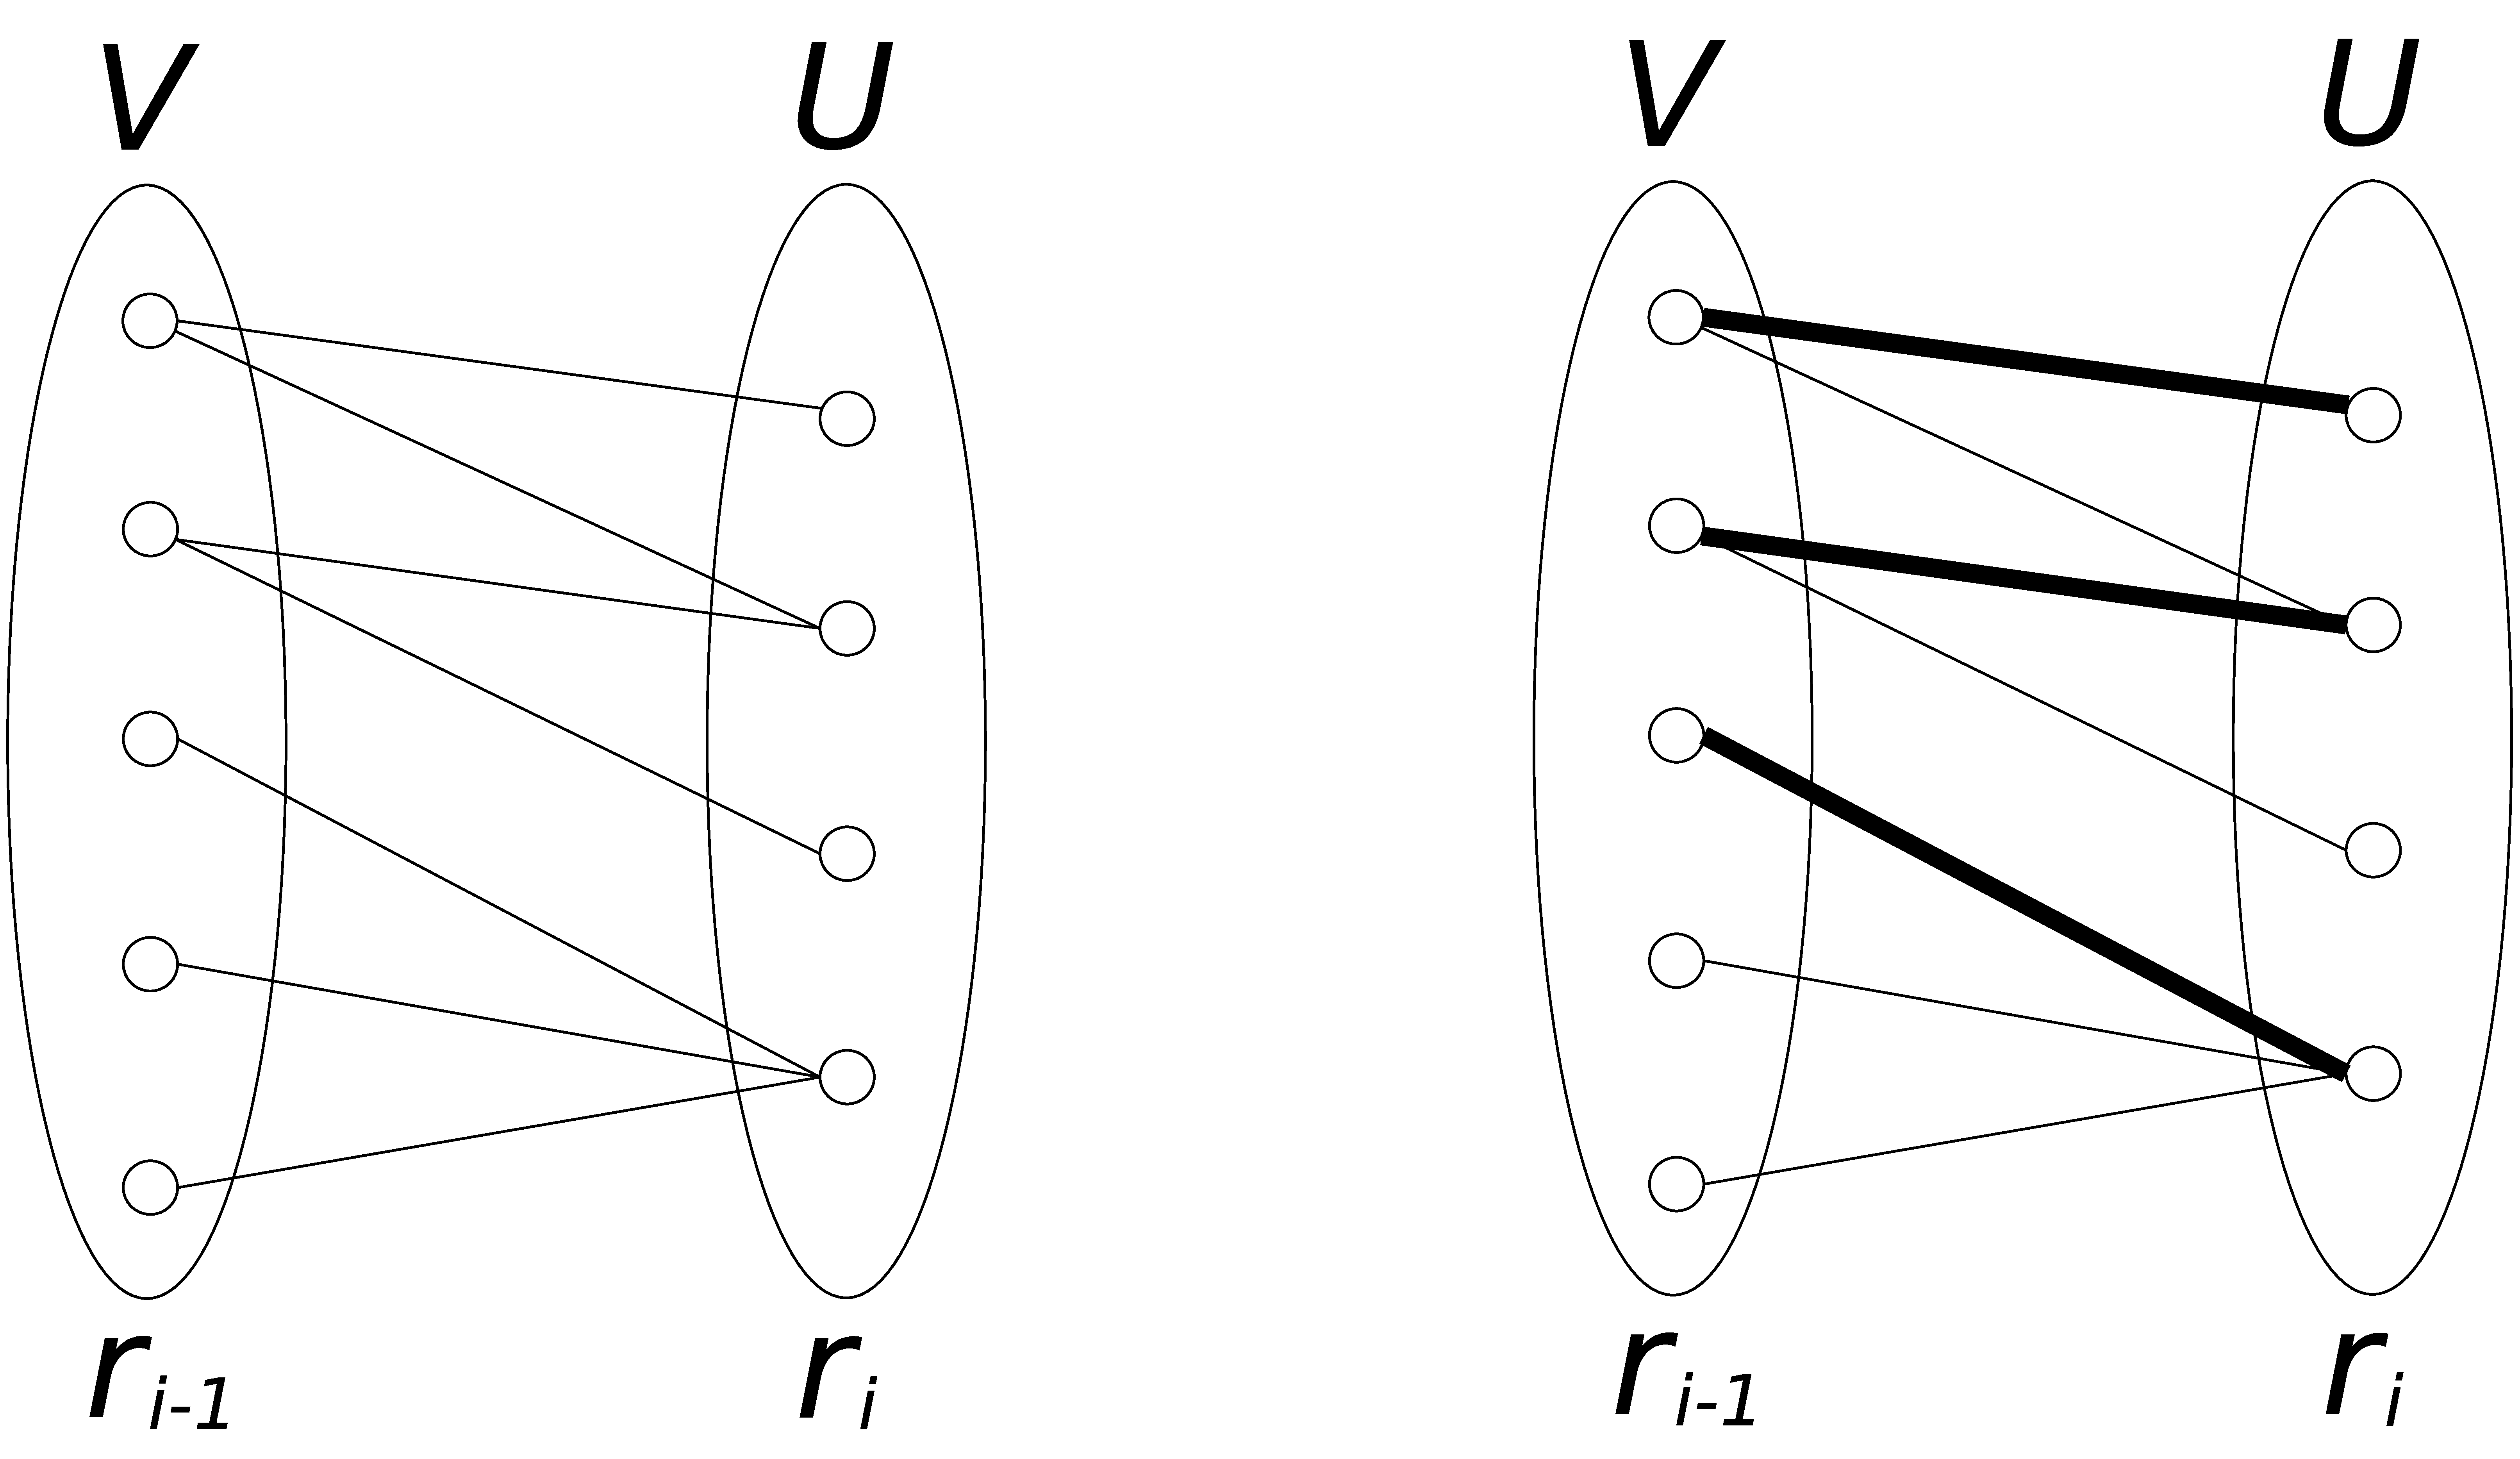
\includegraphics[height=4cm]{bipartite}
    \bicaption[fig:bigraph]{二分图}{一个二分图的例子和它其中一中匹配(被加粗的边)}{Bipartite Graph}{An example of bipartite graph and one of its matching (bold edges)}
\end{figure}
\begin{defn}[图的匹配]
    设$G(V,E)$是一个无向图,如果一个边集$M\subseteq E$中的边两两不相邻(即任意两条边不存在公共的顶点),则成$M$是$G$的一个匹配。
\end{defn}
图\ref{fig:bigraph}中的例子$G(U,V,E)$是一个典型的二分图。我们可以看到所有的边都横跨在两个点集$U,V$之间,而点集的内部不存在任何的边。
在二分图理论中最著名的问题莫过于“二分图最大匹配”问题\citen{west2001introduction},其旨在二分图$G(U,V,E)$中寻找一个最大的匹配$M$。
为了计算最大匹配的值$|M|$,我们需要引入组合数学中著名的霍尔定理\citen{hall1935representatives}的一个拓展:
\begin{thm}[霍尔定理\cite{hall1935representatives}的一个拓展]
    在一个二分图$G(U,V,E)$中,取$U$中的一个子集$X\subseteq U$,记$\Gamma(X)$为$X$的“邻居”,即所有$V$中与$X$中点相邻的点的集合。
    令$\delta(U)=max_{X\subseteq U}\{|X|-|\Gamma(X)|\}$,则有:
    $$MaxMatching(G)=|U|-\delta(U)$$
    \label{thm:hall}
\end{thm}
为了建立轮AKI问题与二分图之间的关系,我们需要这样思考:$r-1$轮和$r$轮的子密钥分别对应子集$V$和$U$中的一个顶点,而这两轮比特之间的一条依赖关系对应横跨$U,V$之间的一条边。
对于给定的子密钥集合$K$(均在$r$轮上),我们把$K$中所有的比特转化成顶点集合$U$,将$K$所依赖的所有$r-1$轮的比特转化为顶点集合$V$,他们之间的依赖关系转化为边集$E$,这样就可以构造出一张二分图$G(U,V,E)$。
这样构造之后,我们重新考虑定理\ref{thm:hall}中的子集$X$(可以视为$K$的一个子比特集合),它的“邻居”$\Gamma(X)$实际上包含了$X$依赖的所有$r-1$轮上的比特,即用$\Gamma(X)$中的所有比特可以推出$X$中的所有比特。
因此,我们可以得出以下引理:
\begin{lem}
    给定一个集中在一轮上的子密钥集合$K$和它的一个子集$X$,令$K'=\Gamma(X)\cup(K\backslash X)$,则$K'$是$K$的一个密钥信息集合。
\end{lem}
\begin{proof}
    由于$\Gamma(X)$可以推出$X$,而$K\backslash X$显然可以推出$K\backslash X$本身,则$K'$可以推出$K$,因此$K'$是$K$的一个密钥信息集合。
\end{proof}
为了找出$K$的实际密钥信息集合,我们需要找到一个最小的密钥信息集合。由于
$$|K'|=|K|-|X|+|\Gamma(X)|=|K|-(|X|-|\Gamma(X)|)$$
又由前文构造出的图$G(U,V,E)$,我们可以得到实际密钥信息集合$K'_{min}$必然满足:
\[
\begin{split}
    |K'_{min}|&=min\{|K|-|X|+|\Gamma(X)|\}\\
              &=|U|-max_{X\subseteq U}\{|X|-|\Gamma(X)|\}\\
              &=|U|-\delta(U)=MaxMatching(G) \qquad\ref{thm:hall}
\end{split}
\]
因此,一个子密钥集合$K$的实际密钥信息的值等于由$U=K$构造出的二分图$G(U,V,E)$的最大匹配的值,且实际密钥信息集合为$K'_{min}=\Gamma(X_{max})\cup(K\backslash X_{max})$,其中$X_{max}$是使$|X|-|\Gamma(X)|$最大的$X$。

\section{AKI-最小割算法}
上一章中提到的单轮加密的AKI只限于计算两轮之间的AKI值,无法将整个密码函数整体考虑。
黄佳琳博士在\citen{Huang_2014}中提到的AKI算法即为每次将密钥依赖路径中的一部分比特同时推至同一轮,考虑与同一轮比特之间的关系,这将会导致一些遗漏,下文将会提到其中的一个反例(该反例同样适用于Lin在\citen{lin2016automatic}提到的密钥桥算法)。
为了寻找一般情况下一个猜测集合的实际密钥信息集合,我们需要将单轮的特殊情况推向多轮的一般情况。
\subsection{一个简单的反例}
如果将猜测集合$K$中大于$r$轮的所有密钥都推到第$r$轮,同时考虑这些密钥与第$r$轮之间的依赖关系,使用上一节提到的二分图匹配算法寻找密钥信息集合,这将会遗漏一些特殊情况:
由于在这种情况下,密钥信息集合只可能取第$r$轮上的比特或是$K$中的比特,完全不考虑$r$轮之后的不在$K$中的比特,这很容易导致遗漏更小的密钥信息集合。
图\ref{fig:counter}提供了一个2轮密钥编排方案的反例,其中$K$为$r_2$轮上的3个比特。
在该反例中,无论是单独考虑$K$与$r_1$轮的密钥还是单独考虑$K$与$r_0$轮的密钥,都无法得出正确的实际密钥信息集合,因为真正的实际密钥信息集合中包含了分布在$r_0$和$r_1$两轮上的不同的比特。
因此,我们需要将所有轮密钥上涉及的比特统一考虑,才不会遗漏这种特殊情况。
\begin{figure}
    \centering
    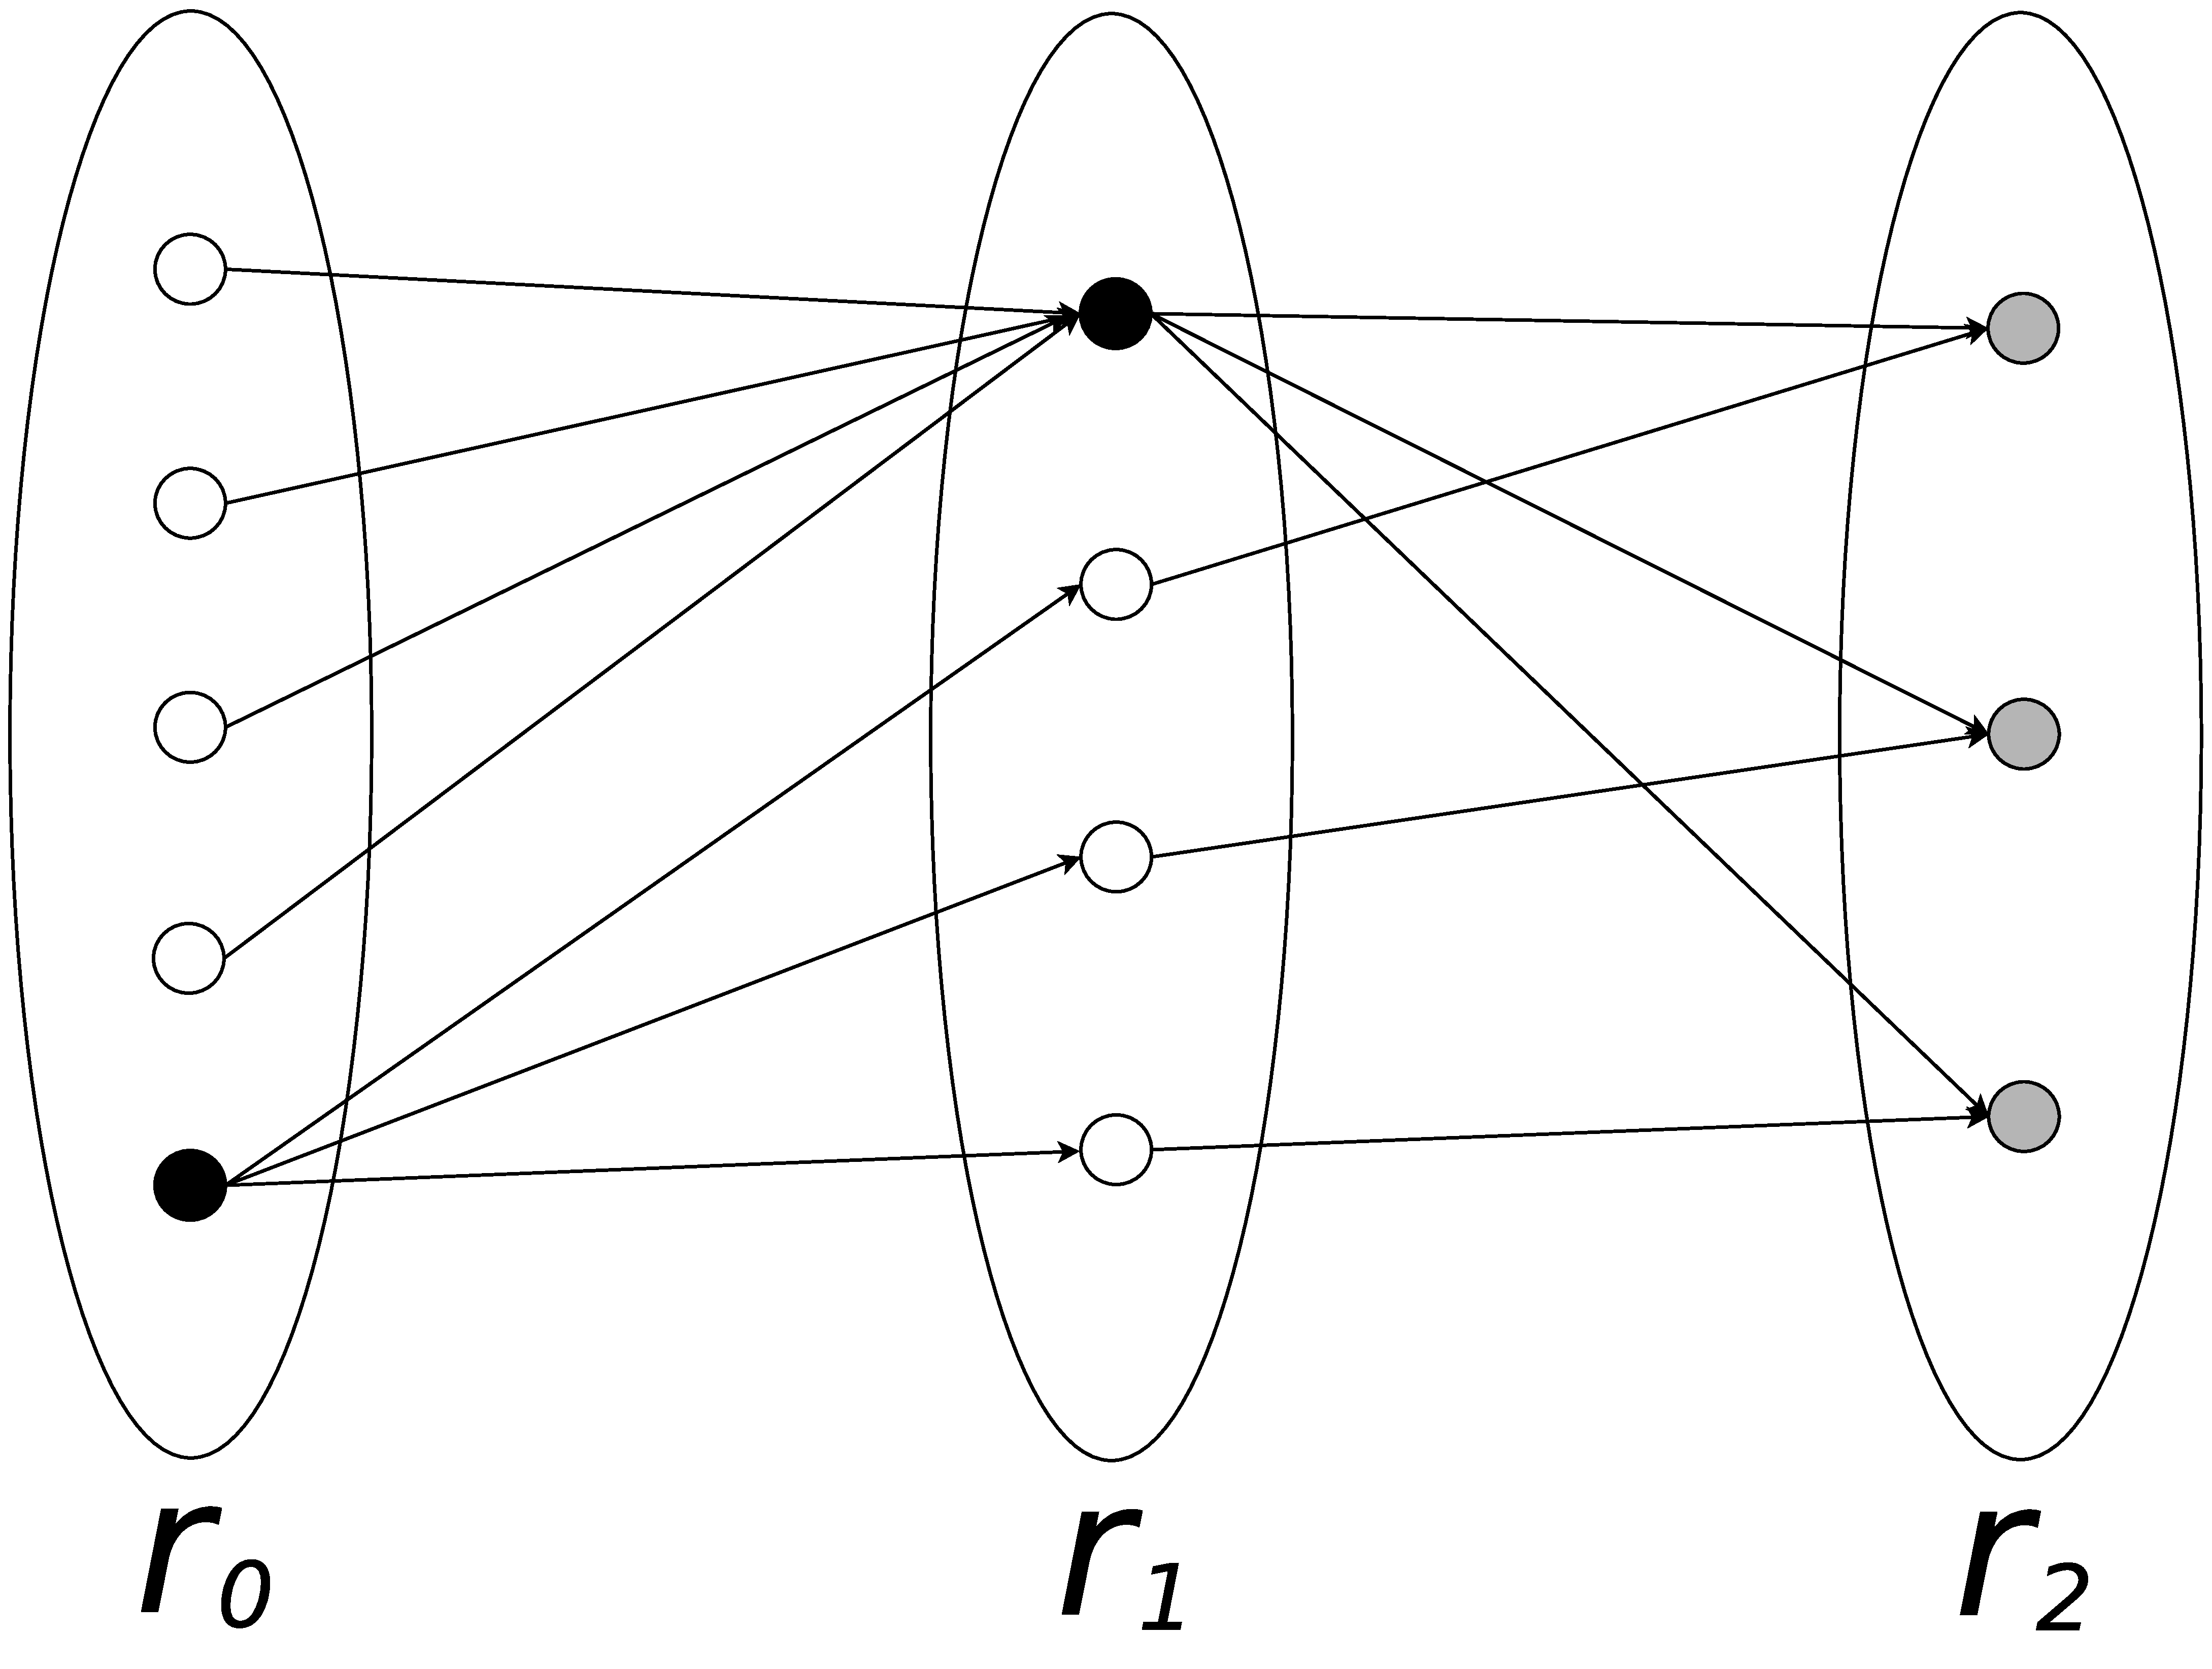
\includegraphics[height=3.3cm]{counter}
    \bicaption[fig:counter]{反例}{一个两轮密钥编排方案的反例,其中灰色的点代表猜测集合$K$,黑色的点是其实际蜜月信息集合。}{Counterexample}{The counterexample with a 2-round schedule. The bits in $K$ are filled with grey and the AKI-set bits are filled with black.}
\end{figure}
\subsection{最大流问题与最大流-最小割定理}
为了将所有轮密钥上的比特统一考虑,我们需要一个适用更加一般的情况的算法。
在图论中,二分图匹配问题是网络流最大流问题的一个特殊情况,因此我们猜想,真正的AKI算法将会使用网络流作为媒介来量化整个密钥编排方案。
在这一节中,我们将简单地介绍最大流问题以及最大流理论中非常重要的一个定理。
\begin{defn}[流量网络]
    一个连通的赋权有向图$G_f(V,E,c)$被成为一个流量网络(或容量网络),其中$c$是弧上的容量,并满足:
    \begin{enumerate}
        \item $c(u,v)$ 代表有向边$e=(u,v)$上的容量。如果$e\notin E$,则$c(u,v)=0$。
        \item 顶点集合中$V$有两个特殊的顶点$s$和$t$分别代表源点与汇点,并满足$\forall(u,v)\in E,u\neq t,v\neq s$(即不存在以t为起始或以s为终点的有向边)。
    \end{enumerate}
\end{defn}
\begin{defn}[流]
    一股流是一个对于所有顶点$u$和$v$都有以下特性的实数函数$f:V^2\rightarrow R$:
    \begin{enumerate}
        \item 容量限制(Capacity Constrains):$f(u,v)\leq c(u,v)$,即弧上的流不能超过该弧的容量;
        \item 斜对称(Skew Symmetry):$f(u,v)=-f(v,u)$,即由$u$到$v$的净流必须是由$v$到$u$净流的相反。
        \item 流守恒(Flow Conservation):除非$u=s$或$u=t$,否则$\sum_{v\in V}f(u,v)=0$,即除了源点与汇点以外的所有点流出的流量为0。
    \end{enumerate}
    流$f$的大小定义为$val(f)=\sum_{u\in V}f(s,u)$。
\end{defn}
最大流问题旨在流量网络$G_f(V,E,c)$中寻找一个最大的流$f$。目前有很多解决该问题的算法,例如Ford-Fulkerson算法\citen{ford1956maximal},预留推进算法,Dinic算法\citen{dinits1970algorithms}等。

最大流问题的对偶问题——最小割问题,同样是十分著名的图论问题之一。
\begin{defn}[割]
    设$S$和$T$为流量网络$G_f(V,E,c)$顶点集合$V$的一个分割,即$S\cup T=V$且$S\cap T=\varnothing$,并满足$s\in S,t\in T$,则称$C=(S,T)$为流量网络$G_f$的一个割。
    其中割$C(S,T)$的大小定义为:
    $$cap(C)=\sum_{(u,v)\in E,u\in S,v\in T}c(u,v),$$
    即为$G_f$中所有从$S$到$T$的弧的容量总和。
\end{defn}
\begin{figure}[htbp]
\centering
    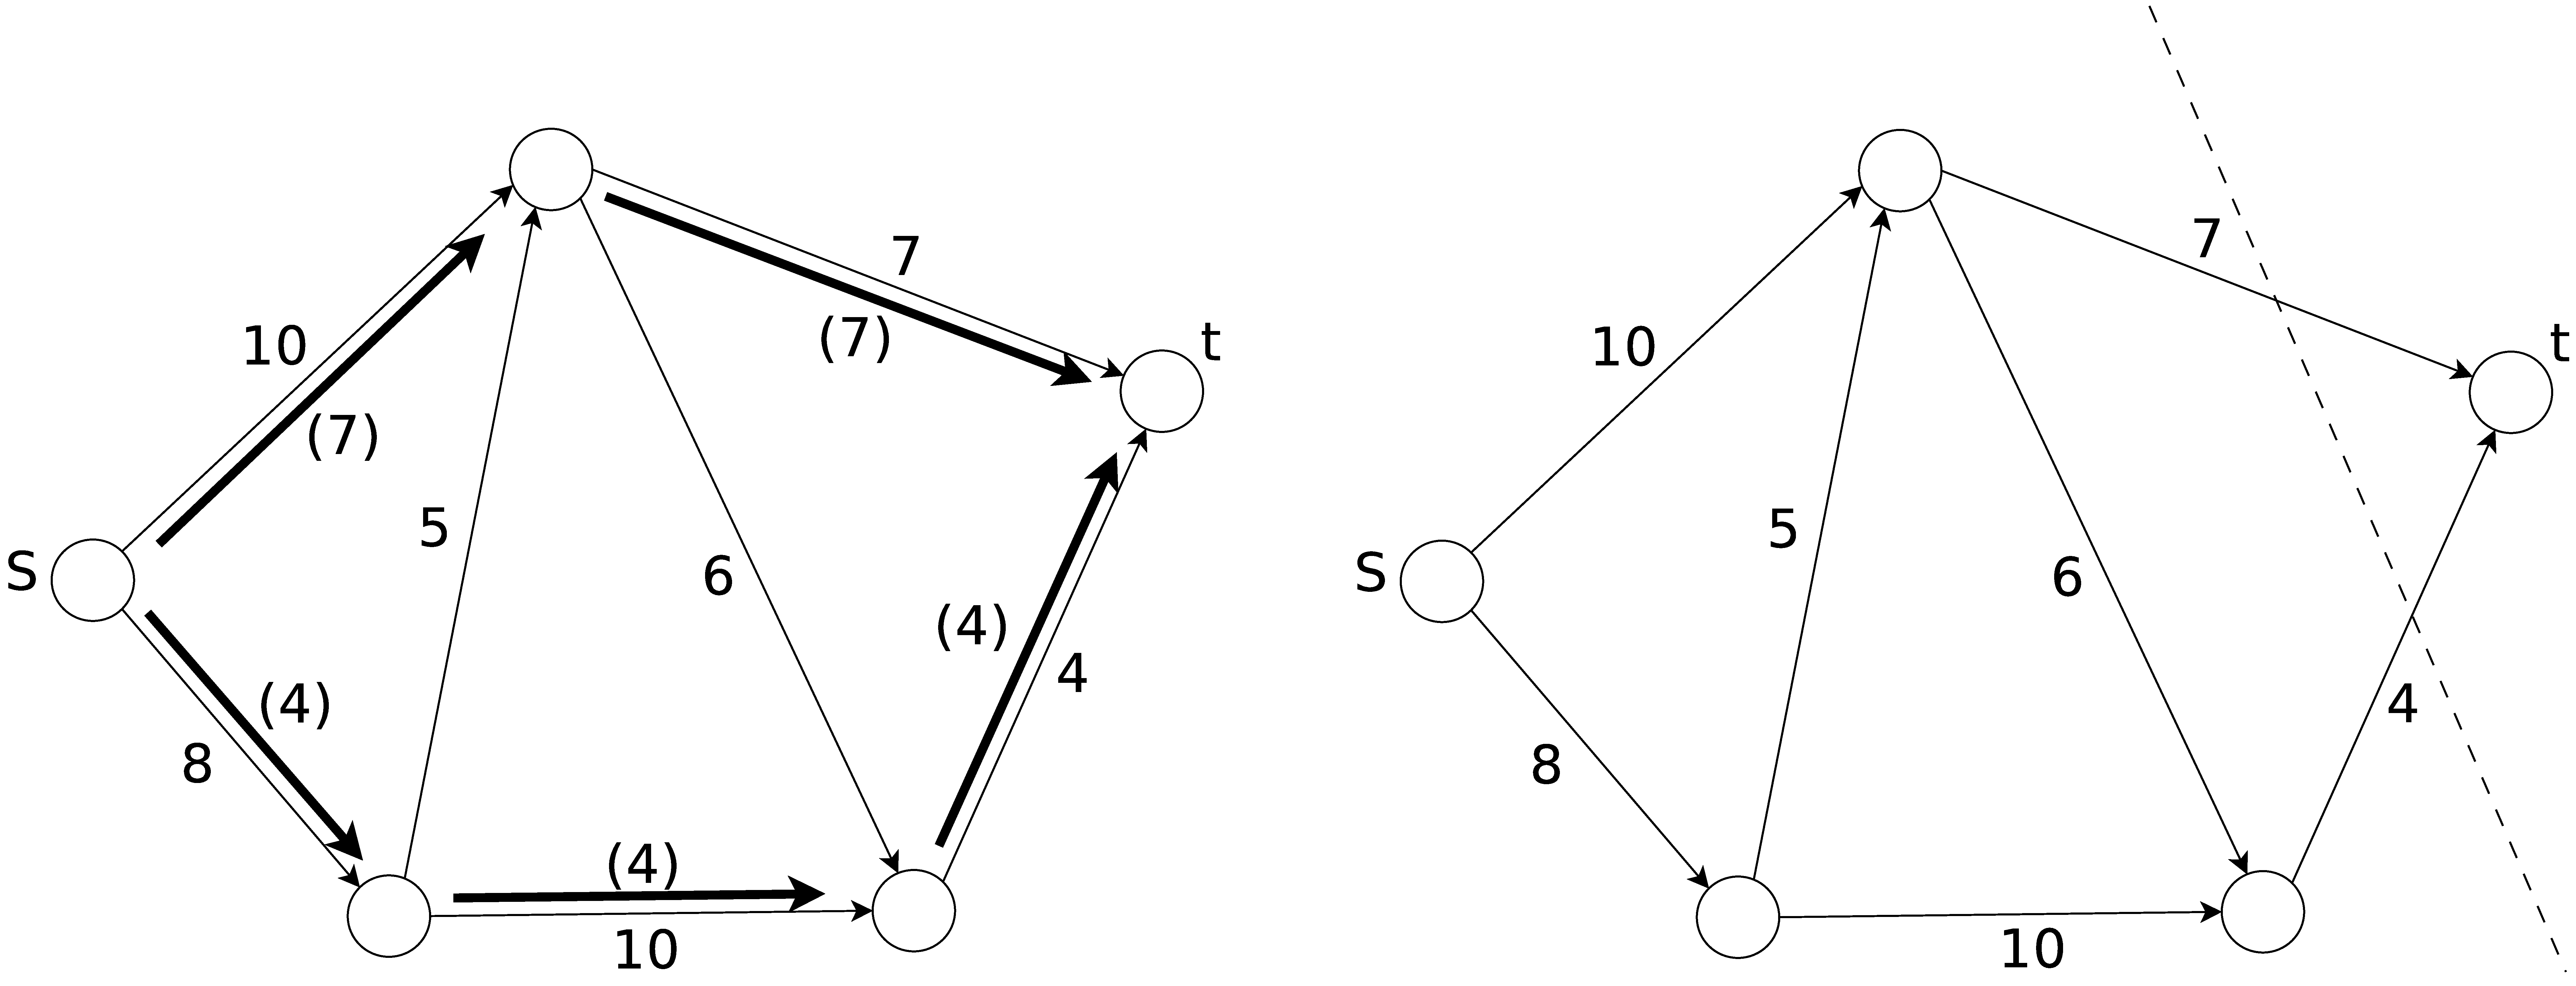
\includegraphics[height=4.5cm]{flowcut}
    \bicaption[fig:flowcut]{最大流与最小割}{一个流量网络的样例中的最大流(左图加粗的边和括号中的数字)和最小割(右图的虚线)}{Max-flow and Min-cut}{An exmaple flow network with its capacities and one of its max-flow (the bold edges and enclosed numbers) and its min-cut (the dotted line)}
\end{figure}
而最大流问题与最小割问题的对偶关系可以由网络流理论中著名的最大流-最小割定理来说明:
\begin{thm}[最大流-最小割定理\citen{papadimitriou19986}]
    在一个流量网络$G_f(V,E,c)$中,最大流的大小等于最小割的大小。
\end{thm}
图\ref{fig:flowcut}中展示了一个同一张图中最大流与最小割的例子。

\section{算法描述}
通过上一节关于最大流与最小割问题的介绍,我们大致了解了最大流与最小割的含义与性质。
在这一节中,我们将介绍一个全新的基于最大流最小割理论的AKI算法——AKI-最小割算法。
该算法旨在将密钥编排方案(用其密钥依赖矩阵$M$表示)和猜测集合$K$转化为一个流量网络$G_f(E,V,c)$,然后在该网络上求最小割来寻找实际密钥信息集合。
\begin{algorithm}[h]
    \caption{流量网络$G(E,V,c)$的构造}
    \begin{algorithmic}[1]
        \Function{Construct}{$K,M$}
            \State $s,t \gets$ new vertex()
            \State $V \gets \{s,t\}$
            \State $K' \gets$ \Call{Get\_Depend\_Bits}{$K,M$}\Comment{将$K$根据依赖关系扩散到所有前轮比特}
            \ForAll {$b\in K'$}
            \State $u_b,v_b \gets$ new vertex()
            \State $V \gets V \cup \{u^b_{in},u^b_{out}\}$
            \State $E \gets E \cup \{(u^b_{in},u^b_{out})\}$
            \State $c(u^b_{in},u^b_{out}) \gets 1$
            \If {$b$是主密钥上的比特}
            \State $E \gets E \cup \{(s,u^b_{in})\}$
            \State $c(s,u^b_{in}) \gets \infty$
            \EndIf
            \If {$b\in K$}
            \State $E \gets E \cup \{(u^b_{out},t)\}$
            \State $c(u^b_{out},t) \gets \infty$ \EndIf
            \EndFor
            \ForAll {$b,b'$是相邻两轮上的比特,且$b'$依赖$b$}
            \If {$u^b_{out}\in V$ and $u^{b'}_{in}\in V$}
            \State $E \gets E \cup \{(u^b_{out},u^{b'}_{in})\}$
            \State $c(u^b_{out},u^{b'}_{in}) \gets \infty$
            \EndIf
            \EndFor
            \State \Return {$G(E,V,c)$}
        \EndFunction 
    \end{algorithmic}
    \label{alg:const}
\end{algorithm}

为了建立密钥比特与流量网络之间的关系,我们使用算法\ref{alg:const}由猜测集合$K$和依赖矩阵$M$构造一个流量网络$G$。
简单来说,除了流量网络中固定的特殊点源点$s$和汇点$t$,我们为每一个猜测比特$K$中的或$K$所依赖的密钥比特$u$建立两个顶点:入点$u_{in}$和出点$u_{out}$,并从入点$u_{in}$引一条容量为1的弧至$u_{out}$。
除了这些容量为1的弧以外,所有的弧均拥有无限大的容量,这些弧分别由以下三种情况建立:
\begin{enumerate}
    \item 从源点$s$到某个处在主密钥上的比特$u$的入点$u_{in}$的弧;
    \item 从某个在$K$中的比特$u$的出点$u_{out}$到汇点$t$的弧;
    \item 分布在连续两轮上的存在依赖关系的两个比特$u$和$v$,后轮的$v$依赖前轮的$u$时,从出点$u_{out}$到$v_{in}$的弧。
\end{enumerate}

由以上的构造可以看出,同一轮比特之间不可能存在弧,只有相邻两轮的比特之间或与源点汇点之间才会存在无穷大容量的弧,这一点性质与\ref{Bigraph}中讨论的二分图的性质十分相似。
因此,我们可以将构造出的流量网络类似的分成$R$个分组,一个分组包含一轮上比特对应的入点与出点,其中$R$是$K$中比特所在的最大的轮数。
图\ref{fig:flow}展示了一个由图\ref{fig:toy}中的玩具密码通过算法\ref{alg:const}得出的流量网络图。
\begin{figure}[htbp]
\centering
    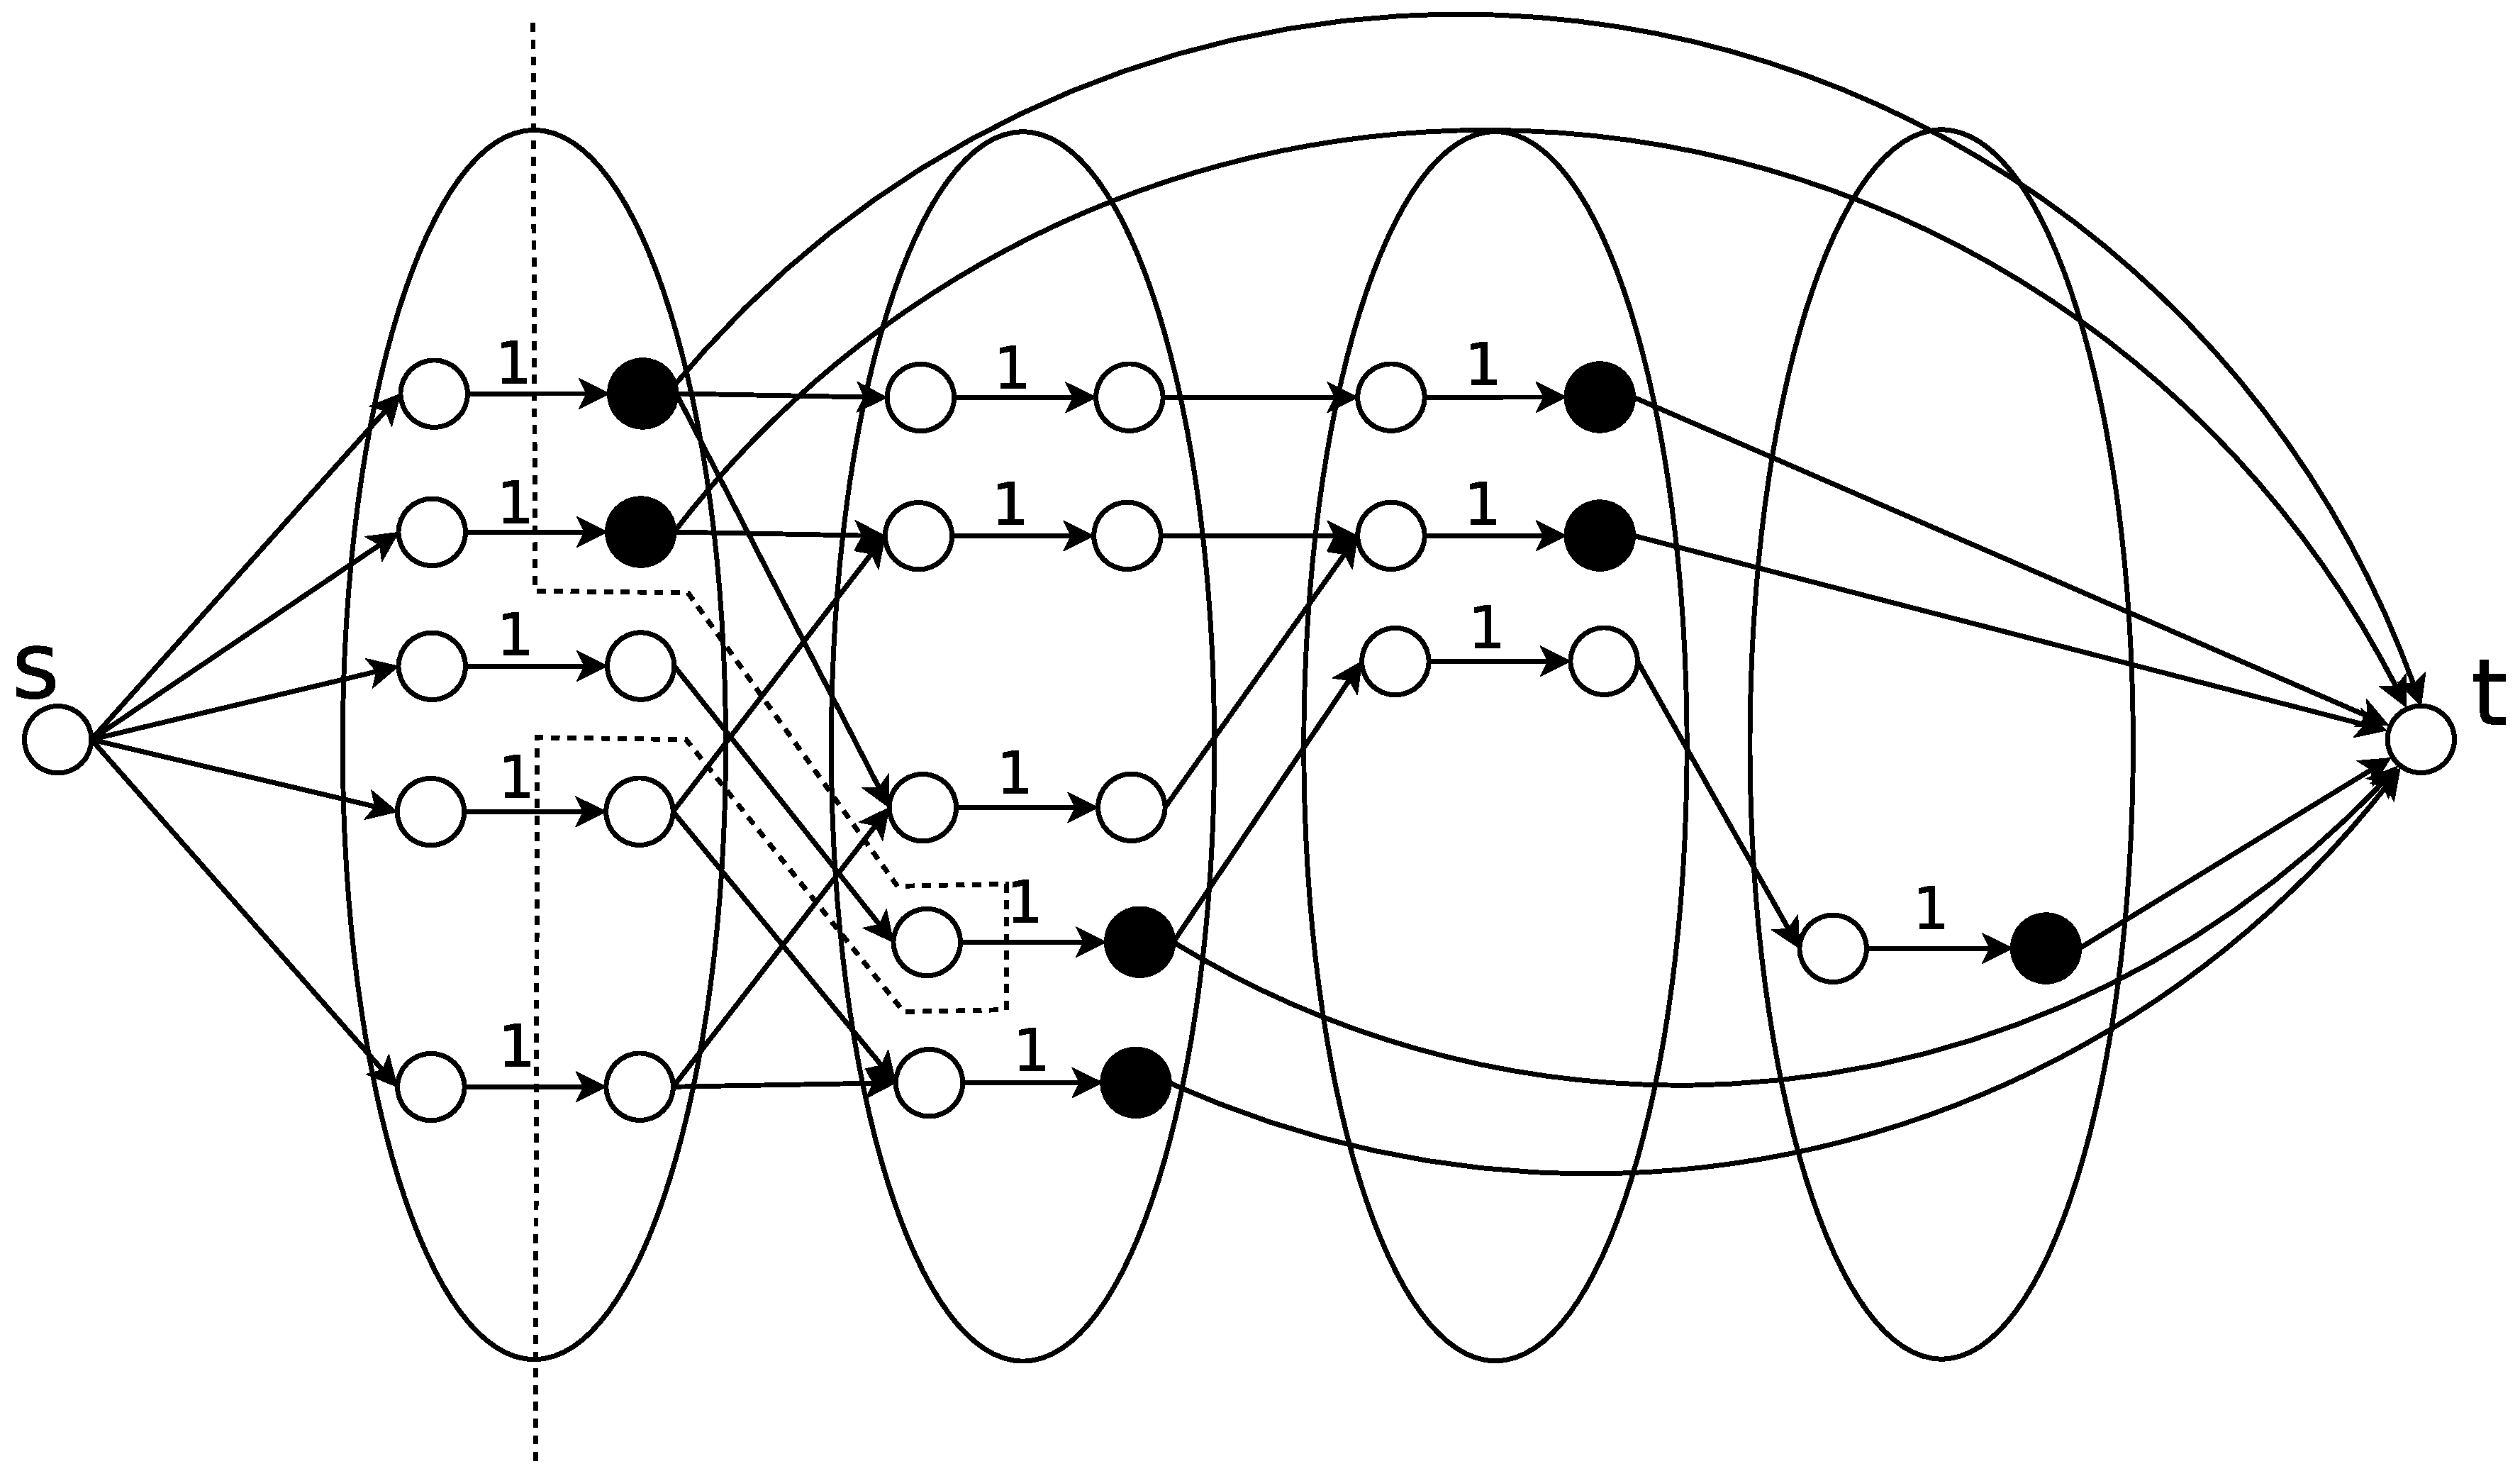
\includegraphics[width=10cm]{flow}
    \bicaption[fig:flow]{构造出的流量网络}{由图\ref{fig:toy}中的玩具密码的例子所构建出的流量网络图。黑色的点代表$K$中的比特,而虚线则是该流量网络的一个最小割。}{Constructed Flow Graph}{One example for the constructed directed flow graph by the Algorithm.~\ref{alg:const} of construction of $G(E,V,c)$ from the example in Fig.~\ref{fig:toy}. The vertices colored in black stands for the bits in $K$, and the dotted line is one of its Min-cut.}
\end{figure}

建立流量网络后,我们只需要对该流量网络应用一个最大流算法,得出的最大流就是$K$的AKI值,而对应的最小割\footnote{一种从最大流中得出最小割的方法是在最大流的残量网络(Residual Network)中找到容量满且两个顶点分别与$s$和$t$连通的边。}中入点与出点被割在两个不同集合中比特构成的集合即为一个实际密钥信息集合。我们称它为AKI-最小割算法\ref{alg:AKI}。
\begin{algorithm}
    \caption{AKI - 最小割算法}
    \begin{algorithmic}[1]
        \Function{GetAKI}{$K,M$}
            \State $G \gets$\Call{Construct}{$K,M$}
            \State $C \gets$\Call{Get\_Min\_Cut}{$G(E,V,c)$}
            \State $K_0 \gets \{u\mid u_{in}\in C.S,u_{out}\in C.T$\}
            \State \Return $K_0$
        \EndFunction
    \end{algorithmic}
    \label{alg:AKI}
\end{algorithm}

\section{算法证明}
在这一节中,我们将对上文提出的AKI-最小割算法\ref{alg:AKI}所得出的实际密钥信息集合$K'_0$的正确性进行证明。
我们将借助一个双向的构造来进行证明:给定一个容量有限的$s-t$割(为了描述方便,我们称这种割为合法割),我们可以构造一个等大小的密钥信息集合;给定一个密钥信息集合,我们可以构造一个等大小的合法割。
\begin{thm}
    假设子密钥比特之间的依赖关系是单向的\footnote{如果要考虑双向关系下的实际密钥信息集合,需要使用解密算法矩阵再次运行算法\ref{alg:AKI}并同时考虑两个集合。注意解密矩阵不一定是加密矩阵的逆。},则算法\ref{alg:AKI}得出的集合就是$K$的最小的密钥信息集合(即实际密钥信息集合)。
\end{thm}
\subsection{合法割$\Rightarrow$密钥信息集合}
给定一个合法$s-t$割$C(S,T)$,其中$s\in S,t\in T$,我们将证明$K_0=\{u\mid u_{in}\in S,u_{out}\in T\}$是一个密钥信息集合,其中$|K_0|=cap(C)$。

首先,由于割$C$是一个合法割,即$C$的容量不为无穷大,且由算法\ref{alg:const}构造出的流量网络$G_f(V,E,c)$中容量为有限的弧都是从入点$u_{in}$到出点$u_{out}$的弧,我们可以由割的容量的定义得到:
$$\begin{aligned}
    cap(C)&=\sum_{u_{in}\in S,u_{out}\in T}c(u_{in},u_{out})\\
          &=\sum_{u_{in}\in S,u_{out}\in T}1\\
          &=|\{u\mid u_{in}\in S,u_{out}\in T\}|\\
          &=|K_0|
\end{aligned}$$

然后我们证明$K_0$是一个密钥信息集合。令$S_0=\{u\mid u_{in}\in S\mbox{ or }u_{out}\in S\}$,即割集$S$中的点所对应的比特的集合;同时令$T_0$为$T$中点所对应的比特的集合。
因为割$C(S,T)$的容量有限,所以不存在弧$(u_{out},v_{in})$,$u_{out}\in S,v_{in}\in T$(否则$c(u_{out},v_{in})$将会倍累计进$cap(C)$)。
注意到$(u_{out},v_{in})$是由$u$与$v$之间的依赖关系所构造出来的弧,且由于$u_{out}\notin T,v_{in}\notin S$我们可以断定$u,v$不属于$K_0$,我们可以得出$T_0\backslash K_0$中的比特不会直接依赖于$S_0\backslash K_0$中的比特,即$T_0\backslash K_0$不会直接依赖于$T_0$。
由此,我们可以有以下证明:

\noindent
\textbf{求证:}$K_0$可以推出$T_0\backslash K_0$中的所有比特。

\noindent
\textbf{证明:}假设存在一个$T_0\backslash K_0$中在第$r_u$轮上的比特$u$无法由$K_0$推出,我们有:
\begin{enumerate}
    \item 考虑第$r_u-1$轮上的比特中必然存在一个比特$v$,$u$直接依赖与$v$而$v$无法由$K_0$推出(否则所有$u$直接依赖的比特都能由$K_0$推出,$u$就可以由$K_0$推出了,这与假设矛盾)。
        由于$u\in T_0\backslash K_0$,$v\in T_0\backslash K_0$($v\in T_0$且$v$不能由$K_0$推出)。
    \item 类似地,考虑$r_u-2$上的比特,我们能由$v$找到一个比特$w\in T_0\backslash K_0$。
    \item 重复以上步骤后,我们能够找到一个在第一轮(主密钥)上的比特$u'$且$u'\in T_0\backslash K_0$。
        但是由于$u'\in T_0\backslash K_0$意味着$u_{in}\in T$,而$s\in S$且$c(s,u_{in})=\infty$,这使得割$C(S,T)$的容量变为无穷大,与假设矛盾。
        因此,假设不成立,即$T_0\backslash K_0$中的所有比特都可以由$K_0$推出。\qed
\end{enumerate}

同时由于$K_0$显然可以推出本身,我们可以得出$K_0$可以推出$T_0$中的所有比特。
根据构造,猜测集合$K$中的所有比特都有出点引出的弧$c(u_{out},t)=\infty$,因此$u_{out}$必然在割集$T$中,即$K\subseteq T$。
因此,$K_0$可以推断出$K$中的所有比特,根据定义,$K_0$是$K$的一个密钥信息集合。

\subsection{密钥信息集合$\Rightarrow$合法割}
给定一个密钥信息集合$K_0$,我们将会按以下步骤在构造出的流量网络$G_f(V,E,c)$中构造出一个合法割$C(S,T)$:
\begin{enumerate}
    \item 对于所有$K_0$中的比特$u$,将$u_{in}$加入割集$S$;
    \item 对于$GetDepend(K_0)$中的比特$u$($K_0$中的某些比特依赖$u$)且$u$不能被$K_0$推出,则将$u_{in}$和$u_{out}$加入割集$S$;
    \item 将$s$加入割集$S$;
    \item 令$T=V\backslash S$,即剩余所有点都加入割集$T$。
\end{enumerate}

根据以上对$C(S,T)$的构造,我们可以得出如果$u_{out}\in S$,则$u$不能被$K_0$推出。
由于$K_0$是$K$的一个密钥信息集合,所有$K$中的比特均可以被$K_0$推出,因此对$\forall u\in K$有$u_{out}\in T$,所以$K\subseteq T_0$。

接下来,我们将由反证法证明割$C(S,T)$是一个合法割。假设$C(S,T)$不合法,即:
$$\exists (u,v),u\in S,v\in T,c(u,v)=\infty$$

我们考虑所有三种容量为无限大的弧:
\begin{enumerate}
    \item $(u_{out},v_{in}),u_{out}\in S,v_{in}\in T$。由于$u_{out}\in S$,我们可以得出$u$不能由$K_0$中的比特推出,因此根据$u$和$v$的依赖关系有$v$也不能由$K_0$中的比特推出。
        而由于$v$不能被$K_0$推出但是$v_{in}\in T$,我们可以根据割$C(S,T)$的第二步构造得出$v\notin GetDepend(K_0)$,因此$v_{out}\in T$。
        在这种情况下,我们可以找到$K$中的至少1比特密钥$u'$不能被$K_0$推出,而我们可以通过以下步骤找到$u'$:
        \begin{enumerate}
            \item 若存在弧$(v_{out},w_{in})\in E$,即$w$直接依赖$v$,我们可以得出$w\notin GetDepend(K_0)$(否则$v$就会在$GetDepend(K_0)$中)。因此根据构造,$w_{in}$和$w_{out}$均会被加入割集$T$,以及$w\notin K_0$(否则$w$就是我们要寻找的比特)。
                因此,$w$不能被$K_0$推出;
            \item 考虑比特$w$,类似地我们可以找到比特$x$有$(w_{out},x_{in})\in E$且$x$不能由$K_0$推出;
            \item 重复以上步骤寻找下一比特,但这个步骤不能无限的循环下去,因为每次寻找到一个新的比特,新的比特所在的轮数都会增加,而根据流量网络$G_f$的构造,这个轮数不能超过$K$中比特所在最大的轮数。
                因此,这个步骤将会在寻找到一个比特$u'$,它的出点$u'_{out}$只引出一条弧$(u'_{out},t)$的时候停止,而这意味着$u'\in K$。
        \end{enumerate}
        因此在这种情况下,$K_0$无法推出$K$中的比特$u'$,这意味着$K_0$不是$K$的一个密钥信息集合,这与我们的假设矛盾。
    \item $(s,v_{in}),v_{in}\in T$。由于$v_{in}\in T$,根据割的构造的第一步我们可以得出$v$不在$K$中。
        同时,考虑到$v$是在第一轮(主密钥)上的,很显然它不能被$K_0$推出,所以由第二步构造我们可以得出$v\notin GetDepend(K_0)$。
        这样,$v$就符合了上述第一种情况中$v$的条件,我们就可以按照第一种情况中的步骤来寻找$K$中的比特$u'$然后得出一个矛盾。
    \item $(u_{out},t),u_{out}\in S$。这种弧存在当且仅当$u\in K$,但是$u_{out}$被加入割集$S$的情况只可能发生在构造的第二步,即$u$不能被$K_0$中的比特推出。
        那么$u$自身就说明了$K_0$不是$K$的密钥信息集合,从而得出了矛盾。
\end{enumerate}

因此我们之前的假设是不成立的,这就证明了$C(S,T)$是一个合法割。为了计算合法割$C(S,T)$的容量$cap(C)$,我们只需要考虑那些容量为1的边,即$u_{in}$和$u_{out}$被分到不同的割集的情况;而根据割$C(S,T)$的构造,将$u_{in}$和$u_{out}$分到两个不同的割集只有可能发生在构造的第一步,即$u\in K_0$。
因此,$cap(C)=|K_0|$。

\subsection{最小割$\Rightarrow$实际密钥信息集合}
给定一个由算法\ref{alg:const}构造出的流量网络$G_f$,我们可以找到它的一个最小割$C_0$。通过上一节中合法割到密钥信息集合集合的构造方式,我们可以构造出$C_0$对应的一个密钥信息集合$K_0$,$|K_0|=cap(C_0)$。

\noindent
\textbf{求证:}$K_0$是一个实际密钥信息集合。

\noindent
\textbf{证明:}假设$K_0$不是一个实际密钥信息集合,而$K'_0$是一个实际密钥信息集合,有$|K'_0|<|K_0|$。
根据密钥信息集合到合法割的构造,我们可以构造出$K'_0$对应的一个割$C'_0$,$cap(C'_0)=|K'_0|$。
注意到$cap(C'_0)=|K'_0|<|K_0|=cap(C_0)$,这意味着$C_0$不是一个容量最小的割,这与之前$C_0$是最小割的条件矛盾,因此假设不成立,$K_0$是一个实际密钥信息集合。\qed

\section{算法时间复杂度分析}
对于一个猜测集合$K$和一个主密钥$n$比特的密钥编排方案的依赖矩阵$M$,令$R$为$K$中比特所在的最大的轮数,则由算法\ref{alg:const}构造的流量网络$G_f$最多拥有$2nR+2$个顶点(每个比特都会构造出两个顶点,而总共最多有$R\dot n$个顶点)和$n+|K|+nR+n^2R$条弧(当$M$是全1矩阵的情况下)。
现有的最大流算法中,高标预流推进的复杂度为$\mathcal{O}(V^2\sqrt{E})$,其中$V$和$E$分别代表顶点数量和边的数量。
因此,AKI-最小割算法的复杂度将为$\mathcal{O}((2nR+2)^2\sqrt{n+|K|+nR+n^2R})=\mathcal{O}(n^3R^{2.5})$,是一个多项式时间。
这保证了对于大多数加密算法来说,我们的AKI-最小割算法能在数秒内给出最终的答案。
